\documentclass[12pt]{article}

\usepackage{a4wide}
\usepackage[colorlinks=true,linkcolor=black,urlcolor=blue,bookmarksopen=true]{hyperref}
\usepackage{bookmark}
\usepackage{fancyhdr}
\usepackage[utf8]{inputenc}
\usepackage[T1]{fontenc}
\usepackage{graphicx}
\usepackage{float}
\usepackage[a4paper,headheight=16pt,scale={0.7,0.8},hoffset=0.5cm]{geometry}
\usepackage{caption}
\captionsetup[figure]{font=small,labelfont=small}


\pagestyle{fancy} % Encabezado y pie de página
\fancyhf{}
\fancyhead[L]{Federico Brasburg - 96653}
\fancyhead[R]{Trabajo Final - Simulacion}
\renewcommand{\headrulewidth}{0.4pt}
\fancyfoot[C]{\thepage}
\renewcommand{\footrulewidth}{0.4pt}

\begin{document}
\begin{titlepage} % Carátula
	\hfill
\includegraphics[width=6cm]{images/logofiuba.jpg}
    \centering
    \vfill
    \Huge \textbf{Simple Model of Spiking Neurons}
    \vskip2cm
    \Large Trabajo Final - Simulacion \\
    Facultad de ingenieria\\ % Curso 1 para el de la tarde y 2 para el de la noche
    \vskip2cm
    \begin{tabular}{ | l | l | } % Datos del alumn
      \hline
      Alumno: & Brasburg, Federico \\ \hline
      Número de padrón: & 96653 \\ \hline
      Email: & federico.brasburg@gmail.com \\ \hline
    \end{tabular}
    \vskip2cm
    \vfill
    \vfill
\end{titlepage}

\tableofcontents % Índice general
\newpage

\section{Absctract}\label{sec:intro}
El objetivo de este trabajo es del replicar los resultados obtenidos en Simple Model of Spiking Neurons - Izhikevich(2003). \cite{paperOriginal} (a partir de ahora llamado "paper original").
El paper original presenta un modelo que tiene la capacidad de reproductir comportamientos conocidos de las neuronas corticales, como por ejemplo el \textit{spiking} (una traduccion bastante desafortunada seria disparada)
o el \textit{bursting} (cuando hay mucho disparos). El modelo propuesto combina la plausibilidad biologica de las dinamicas de Hodgkin–Huxley \cite{HodgkinHuxley} y la eficiencia computaciones de las neuronas de integracion y disparo.
Estas ultimas neuronas son las que se utilizand para generar modelos de Machine Learning. Usango el modelo propuesto se puede simular miles de neuronas coritcales de disparo con una resolucion de 1ms utilizando cualquier PC (personal computer).
Por fuera del paper original, se probó el modelo propuesto con diferentes paramentros y distintas cantidades neuronas conectadas.
\\ \\
Palabras clave: Bursting, Hodgkin–Huxley, PCNN, neuronas de integracion y disparo, spiking, corteza cerebral.

\section{Introducción}
Para entender como funciona el cerebro humano, se necesita combinar estudios experimentales sobre sistemas nerviosos de animales y humanos con simulaciones numericas de gran escala de modelos cerebrales.
Al momento de desarrollar modelos de neuronas spiking, se tienen siempre dos requerimientos que son aparentemente mutualmente excluyentes sobre cada neurona:
\begin{enumerate}
    \item Tienen que ser computacionalmente simples
    \item Tienen que tener la capacidad de producir patrones de disparos mostrados por neuronas biologicas reales.
\end{enumerate}

Usar modelos que sean biofisicamente semejantes a los de Hodgkin–Huxley es computacionalmente imposible, ya que solo se pueden simular muy pocas al mismo tiempo en tiempo real. Por el otro lado, usar un modelo
puramente con neuronas que integren y disparen es muy efectivo computacionalmente pero es totalmente irrealista y es incapaz de generar las dinamicas de las neuronas reales como el spiking o el bursting.

En el paper original, se presenta un modelo simple de spiking que es bilogicamente plausible al de Hodgkin–Huxley y es computacionalmente eficiente como el de integracion y disparo.
El modelo propuesto solo toma 4 parametros y con eso solo es capaz de reproducir los comportamientos de spiking, bursting y muchos mas conocidos de neuronas corticales reales. En la Fig 1 se puede observar
algunos comportamientos conocidos reproducidos en la corteza cerebral de una rata. \\ \\

\newpage

\begin{figure}
    \centering
        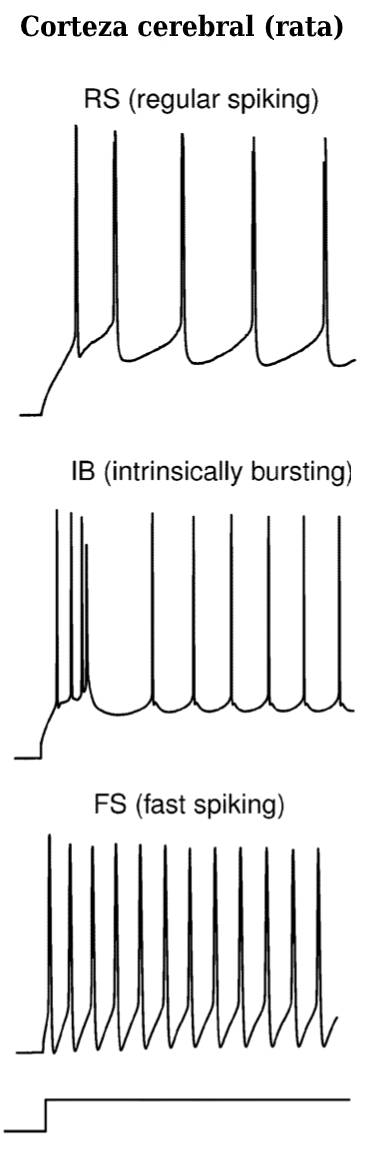
\includegraphics[height=10cm]{images/rata.jpg}
    \caption[fontsize=2pt]{Imagen obtenida del paper original. Se pueden apreciar tres comportamientos conocidos como lo son el regular spiking (RS), el intrinsically bursting (IB) y el fast spiking (FS) en la cortez de una rata}
\end{figure}

El modelo completo fue publbicado por primera vez en \cite{modeloPrimero} en una forma trigonometrica. En este paper se presenta en una forma mas adecuada para simulaciones a gran escala

\section{El Modelo}
Las metodologias de bifurcacion \cite{bifurcacion} nos permiten reducir el modelo neuronal de Hodgkin-Huxley a un sistema bidimensional de ecuaciones diferenciales ordinarias:
\begin{equation}
    \frac{dv(t)}{dt} = 0.04 v(t)^2 + 5 v(t) + 140 - u(t) + I\\
\end{equation}
\begin{equation}
    \frac{du(t)}{dt} = a(b v(t) - u(t))
\end{equation}
Ademas, a $(1) \ y  \ (2)$ le agregamos la regla:
\begin{equation}
    Si \ v(t) >= 30 mV,\ entonces \
        v(t) = 30 \ y \ u(t) = u(t) + d
\end{equation}
Los parametros del sistema son $a, b, c \ y \ d$. $t$ es el tiempo. \\ \\

La variable $v(t)$ representa el potencial de la neurona (medido en mV) y $u(t)$ representa la variable de recuperacion de la neurona,
que cuenta las activaciones de los iones $K^{+}$ y la desacativacion de los $Na^{+}$, ademas aporta negativamente a $v(t)$ \\

Se dice que sucede un \textit{spike} cuando $v(t)$ es mayor a 30mV. Luego de un spike, el voltaje de la membrana ($v(t)$) y la variable de recuperacion ($u(t$)) son reiniciadas de acuerdo a $(3)$.
A cada neurona la estimula una corriente sinaptica que se ve representada en el sistema de ecuaciones en la variable $I$ (que puede ser una funcion dependiente del tiempo o constante).

La parte de $0.004v(t)^2 + 5v(t) + 140$ fue obtenida adecuando las dinamicas del inicio de un spike de una neurona cortical, por lo que mV es la escala para $v(t)$ y $ms$ para el tiempo.
El potencial de reposo (cuando un spike no esta sucediendo) ronda los -70 y -60 mV dependiendo del valor de $b$. Como la mayoria de las neuronas reales, el modelo no tiene un limite fijo (llamamos limite al voltaje del cual parte un spike).
Dependiendo del historial de spikes de la neurona el potencial limite podria ser tan bajo como -55 mV o tan alto como -40 mV.
Los parametros tienen los siguientes significados:
\begin{itemize}
    \item El parametro $a$ describe la escala de tiempo para la varible de recuperación ($u(t)$), por lo que un $a$ chico va a ser que la recuperacion de un spike sea mas lenta. Un valor normal es $a = 0.02$
    \item El parametro $b$ describe la sensitividad de la variable de recuperación a la fluctiación del limite de potencial de la membrana. Mayores valores de $b$ acoplan a $v(t)$ y a $u(t)$ fuertemente dando como resultado
posibles oscilaciones de sublimites y dinamicas de spiking con un limite bajo. Un valor normal es $b = 0.$. El caso $b < a)$ corresponde a una bifurcacion saddle-node del estado de reposo \cite{modeloPrimero}
    \item El parametro $c$ es el valor que se le asigna al potencial de la membrana ($v(t)$) luego de un spike. Un valor normal es el de $c = -65 mV$.
    \item El parametro $d$ es el valor que se le agrega a la variable de recuperacion ($u(t)$) luego de un spike. Un valor normal es el de $d = 2$.
\end{itemize}

Distintas combinaciones de parametros resultan en distintos patrones intrinsecos de disparos, incluidos los conocidos de las neuronas corticales ya mencionados y de las neuronas talamicas (del talamo).
Una posible extension del modelo propuesto es el de tratar $u(t), a$ y $b$ como vecores y usar $\sum{u}$ en lugar de $u$ para el voltaje. Esto sirve para tener en cuenta conductancias lentas con multiples esccalas de tiempo, pero el autor del paper considera que esta extensión es innecesaria para las neuronas corticales.

\section{Resolucion de la ecuacion diferencial}

Esta es una sección que no es parte del paper original pero me parecio importante de contar como hice las simulaciones. Para comenzar se intentó resolver el sistema de ecuaciones diferenciales con python con la libreria $simpy$ \cite{Sympy}
pudiendo llegar a una solucion para ambas
ecuaciones ($v(t)$ y $u(t)$), se utilizó el sistema original del paper y se tomo como condiciones iniciales las del reset luego de un spike de ambas funciones.
Luego se presentó la dificultad de que dicha solucion tambien tenga en cuenta la regla $(3)$ del sistema original, lo cual resulto imposible e hizo que se tenga que buscar otra solución. \\ \\
Finalmente, se adoptó como solución una encontrada utilizando la definición de derivada. La definición es la siguiente: \\
\begin{equation}
    f'(x) = \lim_{h \to 0} \frac{f(x + h) - f(x)}{h}
\end{equation}
\\
Luego se aproximó de la siguiente manera utilizando el metodo de Euler \cite{Euler}:
\begin{equation}
    f'(x) \approx \frac{f(x + h) - f(x)}{h}
\end{equation}

Luego se utilizó $(5)$ para obtener las siguientes funciones ($h$ es la resolución del sistema, en este caso va a ser 0.1ms):
\begin{equation}
    v(t + h) \approx h(0.04 v(t)^2 + 5 v(t) + 140 - u(t) + I) + v(t)
\end{equation}
\begin{equation}
    u(t + h) \approx h(a(b v(t) - u(t))) + u(t)
\end{equation}

Se puede apreciar claramente que dichas ecuaciones no son la solución al sistema de ecuaciones diferenciales. Lo unico que proveen es, partiendo de valores iniciales $v_0$ y $u_0$,
la serie de valores $u_0,...,u_n$ y $v_0,...,v_n$. Para simular solo necesitamos dichas series, no es necesaria la función solución, por lo que se dió como aceptable dicho resolución.

\section{Diferentes tipos de dinamicas}

La siguiente sección va a hablar sobre los distintas patrones que se ven en las neuronas y vale la pena destacar que cada simulación se realizo con los valores
mencionados en el paper original y resolución de (0.1 ms). \\

Las neuronas neocorticales del cerebro mamifero pueden ser clasificadas en diferentes tipos de acuerdo al patron de spiking y bursting visto en estudios intracelulares. \\

\subsection{Celulas corticales exitatorias}
Todas las celulas corticales exitatorias pueden ser divididas en tres clases \cite{firingPatters} \cite{chatteringCells}:

\newpage
\subsubsection{Regular spiking (RS)}
fede
\newpage

\section{Referencias}

\begin{thebibliography}{9}

\bibitem{paperOriginal}
Izhikevich
\textit{Simple Model of Spiking Neurons}. (Ingles) 2003

\bibitem{HodgkinHuxley}
Martin Pospischil. Maria Toledo-Rodriguez. Cyril Monier. Zuzanna Piwkowska. Thierry Bal. Yves Frégnac. Henry Markram
\textit{Minimal Hodgkin–Huxley type models for different classes of cortical and thalamic neurons}. (Ingles) 2008

\bibitem{modeloPrimero}
Int. J. Bifurc.
\textit{Neural excitability, spiking and bursting}. (Ingles) 2000

\bibitem{bifurcacion}
E. M. Izhikevich.
\textit{Dynamical Systems in Neuroscience: The Geometry of Excitability and Bursting}. (Ingles) A ser publicado

\bibitem{Euler}
Euler.
\textit{Método de Eurler}. \url{https://en.wikipedia.org/wiki/Euler_method}

\bibitem{Sympy}
\textit{Sympy}. \url{https://docs.sympy.org/latest/index.html}

\bibitem{firingPatters}
B. W. Connrs y M. J Gutnick.
\textit{Intrinsic firing patterns of diverse neocortical neurons}. (Ingles) Trends in Neurosci., vol. 13, pp. 99-104, 1990.

\bibitem{chatteringCells}
C. M. Gray y D. A. McCormick.
\textit{Chattering cells: superficial pyramidal neurons contributing to the generation of synchronous oscillations in the visual cortex}. (Ingles) Science. vol 274, no. 5284, pp 109-113, 1996.

\end{thebibliography}

\end{document}
